\documentclass{ansjournal}

\usepackage{microtype}                     % Improve typography
\usepackage{amsmath, mathtools}             % AMS Math extensions
\usepackage{booktabs}                      % Improved table spacing
\usepackage{siunitx}
\usepackage{breqn}
\usepackage{nicefrac}
\usepackage{multirow}
\usepackage{enumitem}
\usepackage{subcaption}
\usepackage{dblfloatfix}
\usepackage{color}
\usepackage{todonotes}
\usepackage{etoolbox}
\usepackage{listings}
\usepackage{color}
\usepackage{bbold}

% Checkmarks
\usepackage{amssymb}% http://ctan.org/pkg/amssymb
\usepackage{pifont}% http://ctan.org/pkg/pifont
\newcommand{\cmark}{\ding{51}}%
\newcommand{\xmark}{\ding{55}}%

% Algorithm constructs
\renewcommand{\thealgorithm}{\thechapter-\arabic{algorithm}}
\newcommand\Algphase[1]{%
\vspace*{-.7\baselineskip}\Statex\hspace*{\dimexpr-\algorithmicindent-2pt\relax}\rule{\columnwidth}{0.4pt}%
\Statex\hspace*{-\algorithmicindent}{#1}%
\vspace*{-.7\baselineskip}\Statex\hspace*{\dimexpr-\algorithmicindent-2pt\relax}\rule{\columnwidth}{0.4pt}%
}
\newcommand{\algrule}[1][.4pt]{\par\vskip.5\baselineskip\hrule height #1\par\vskip.5\baselineskip}

\newcommand{\code}[2]{
  \subsection*{#1}
  \lstinputlisting{#2}
}

\lstset{
  basicstyle=\footnotesize\ttfamily,
  columns=fullflexible,
  showstringspaces=false,
  commentstyle=\color{gray}\upshape,
  frame=single,
  xleftmargin=0.8in,
  xrightmargin=0.8in
}

% Patch to make equation autoref counter work
\makeatletter
\patchcmd\eq@setnumber{\stepcounter}{\refstepcounter}{}{%
  \errmessage{Patching \noexpand\eq@setnumber failed}%
}
\makeatother

\hypersetup{colorlinks=true,
  pdftitle={Multi-Group Cross Section Generation with the OpenMC Monte Carlo Particle Transport Code},
  pdfauthor={William Boyd, Adam Nelson, Paul Romano, Samuel Shaner, Benoit Forget and Kord Smith}}

\title{Multi-Group Cross Section Generation with the OpenMC Monte Carlo Particle Transport Code}

\author[a]{William Boyd\footnote{Email: \href{mailto:wboyd@mit.edu}{wboyd@mit.edu}}}
\author[b]{Adam Nelson}
\author[c]{Paul K. Romano}
\author[a]{Samuel Shaner}
\author[a]{Benoit Forget}
\author[a]{Kord Smith}

\affil[a]{Massachusetts Institute of Technology, Department of Nuclear Science
  and Engineering, 77 Massachusetts Avenue, Building 24, Cambridge,
  Massachusetts 02139}
\affil[b]{Something}
\affil[c]{Argonne National Laboratory, Mathematics and Computer Science
  Division, 9700 South Cass Avenue, Lemont, Illinois 60439}


%%%%%%%%%%%%%%%%%%%%%%%%%%%%%%%%%%%%%%%%%%%%%%%%%%%%%%%%%%%%%%%%%%%%%%%%%%%%%%%
\abstractText{Abstract here}
%%%%%%%%%%%%%%%%%%%%%%%%%%%%%%%%%%%%%%%%%%%%%%%%%%%%%%%%%%%%%%%%%%%%%%%%%%%%%%%

\keywordsText{Monte Carlo neutron transport, multi-group cross section generation}

\begin{document}

\maketitle

%%%%%%%%%%%%%%%%%%%%%%%%%%%%%%%%%%%%%%%%%%%%%%%%%%%%%%%%%%%%%%%%%%%%%%%%%%%%%%%
\section{Introduction}
\label{sec:intro}
%%%%%%%%%%%%%%%%%%%%%%%%%%%%%%%%%%%%%%%%%%%%%%%%%%%%%%%%%%%%%%%%%%%%%%%%%%%%%%%

The past two decades have seen growing interest in Monte Carlo (MC) as a means to generate multi-group cross section (MGXS) libraries. Most MC-based MGXS generation schemes to date focus on generating few-group constants for coarse mesh diffusion codes. These schemes aim to improve the accuracy of standard diffusion codes for analysis of atypical core configurations for which the simplifications made by multilevel deterministic MGXS generation methods are not necessarily applicable. These efforts replace the separate resonance self-shielding and deterministic lattice physics calculation steps in multistep approaches with fully detailed MC calculations of each assembly to compute the few-group constants needed by whole-core diffusion codes. The widely used Serpent code\cite{leppanen2015serpent} has led this trend over the past decade, and a few authors have applied the MCNP\cite{pounders2006stochastically} and McCARD\cite{shim2008generation} codes in a similar fashion. This paper presents new capabilities introduced in the OpenMC\cite{romano2015openmc} particle transport code for multi-group cross section generation for fine-mesh multi-group neutron transport applications.

This paper is organized as follows. \cref{sec:mg-theory} summarizes the key multi-group constants required by deterministic multi-group codes. \cref{sec:mgxs-mc} details the mathematical formulation for stochastic integration of each of the multi-group constants currently computable by OpenMC. \cref{sec:openmc} highlights the core OpenMC features that provide the foundation for the \texttt{openmc.mgxs} module for MGXS generation introduced in \cref{sec:design}. \cref{sec:validate} uses the OpenMOC\cite{boyd2014openmoc} multi-group transport code to validate the MGXS generated by OpenMC. \cref{sec:conclusions} summarizes the conclusions.

%%%%%%%%%%%%%%%%%%%%%%%%%%%%%%%%%%%%%%%%%%%%%%%%%%%%%%%%%%%%%%%%%%%%%%%%%%%%%%%
\section{OpenMC Core Features}
\label{sec:openmc}
%%%%%%%%%%%%%%%%%%%%%%%%%%%%%%%%%%%%%%%%%%%%%%%%%%%%%%%%%%%%%%%%%%%%%%%%%%%%%%%

The preceding section outlined the procedures for estimating multigroup cross sections based on flux and reaction rate tallies from a Monte Carlo code. It is conceptually simple to use a Monte Carlo code to compute these tallies and report macroscopic or microscopic multigroup cross sections as part of the output of the code. Indeed, this is the approach adopted by the Serpent Monte Carlo code\cite{leppanen2016homog}. The MGXS generation framework implemented in OpenMC takes a fundamentally different and lightweight approach: instead of using the transport kernel to directly compute and report MGXS, the standard output of the code includes only flux and reaction rate values. After a simulation is complete, the MGXS are calculated as a post-processing task on the reported tallies by a Python application programming interface (API).

OpenMC is an open source Monte Carlo particle transport code that is intended primarily for use in neutron criticality calculations. It can simulate three-dimensional models using constructive solid geometry. It also supports both continuous-energy and multigroup cross section data in a native HDF5\cite{koranne2011hdf5} data format\cite{romano2017epjwoc} that can be generated from ACE files. The following sections summarize OpenMC's tally system and Python API, which form the foundation for the MGXS generation module presented in \cref{sec:design}. 

This section provides a high-level overview of the software engineering design, along with the computational constraints which guided these design choices. The following subsections are intended to provide enough detail for OpenMC users to understand how to efficiently use the MGXS generation module and/or make contributions to the open source codebase. In addition, it is the authors' hope that the details provided here may be of value to developers of other Monte Carlo codes to readily reproduce the MGXS generation methods implemented in OpenMC.

%%%%%%%%%%%%%%%%%%%%%%%%
\subsection{Tally System}
\label{subsec:tallies}

OpenMC features a flexible, low-overhead tally system that enables users to obtain physical results of interest. Tallies are defined by combinations of \emph{filters} and \emph{scores}. Each filter limits what events can score to the tally based on the phase space variables. For example, a filter could limit scoring events to particles traveling within a specified cell or a specified range of pre-collision energies. Each score identifies a physical quantity to be scored when an event occurs that matches the specified filters. Filters correspond to the limits of integration and scores correspond to the integrand itself in \cref{eqn:inner-prod}:

\begin{equation}
\langle \Sigma_x, \psi \rangle = \underbrace{\int_{V} \int_{S} \int_{E}}_{\text{filters}} \underbrace{\Sigma_{x}(\mathbf{r},E)\psi(\mathbf{r},E,\mathbf{\Omega})}_{\text{scores}} \mathrm{d}E\mathrm{d}\mathbf{\Omega}\mathrm{d}\mathbf{r}.
\end{equation}

In addition to filters and scores, one can obtain reaction rates for individual nuclides by specifying a list of nuclides. Each tally definition is permitted to have multiple filters, multiple scores, and multiple nuclides. Additionally, the estimator used to score events can be specified on a per tally basis.

A wide range of filters and scores have been implemented as of the version 0.10.0 release of OpenMC\cite{openmc-090}. The available filters can generally be categorized as follows:
\begin{itemize}[noitemsep]
\item \emph{Spatial domain}: Tally events by universe, material, cell, mesh
\item \emph{Energy domain}: Tally events based on both incoming and outgoing particle energy
\item \emph{Angle domain}: Tally events based on a particle's polar and azimuthal direction or scattering angle
\item \emph{Energy function}: Multiplies tally scores by an arbitrary function of incident energy
\item \emph{Delayed group}: Tally events that produced neutrons in particular delayed groups
\end{itemize}
The available scores in version 0.10.0 include particle flux, all individual reaction rates, neutron production from fission (total, prompt, or delayed), Legendre and spherical harmonic scattering moments, spherical harmonic flux moments, inverse velocity, recoverable fission energy release, and inverse decay constant-weighted delayed neutron precursor production rate. Taken together, these filters and scores permit all inner products identified in \cref{tab:tally-types} to be estimated via tallies in OpenMC.

%%%%%%%%%%%%%%%%%%%%%%%
\subsection{Python API}
\label{subsec:pyapi}

A fully featured Python API enables programmatic pre- and post-processing for OpenMC\cite{boyd2016bigdata}. The API makes it possible to write a single dynamic Python script to specify the simulation parameters, execute the simulation, and analyze the resultant tally dataset. In addition, the API makes it possible to leverage the extensive ecosystem of Python packages for scientific computing alongside OpenMC in a simulation workflow. OpenMC's dynamic object-oriented data processing model---fusing the geometry and materials configuration with tallied data---enables the rapid calculation, indexing, and storage of MGXS from tallies over specified spatial domains. This section describes two features developed for the API to support OpenMC's MGXS generation module.


%%%%%%%%%%%%%%%%%%%%%%%%%%%%%%%%
\subsubsection{Tally Merging and Slicing}
\label{subsubsec:tally-slice-merge}

Two useful and related features in the OpenMC Python API for MGXS generation are \emph{tally merging} and \emph{tally slicing}, as depicted in \cref{fig:tally-merge-slice}. It is intuitively useful to create separate \texttt{Tally} objects for each spatial domain and reaction type when generating the OpenMC inputs necessary to compute MGXS. However, this approach necessarily leads to a large number (e.g., 10$^2$ -- 10$^4$) of distinct tally objects for large, complex geometries, which poses a computational bottleneck since the overhead to tally in OpenMC scales as $\mathcal{O}(N)$ for $N$ tallies\footnote{Note that $N$ refers to the number of tally definitions, each of which can contain multiple filters, nuclides, and scores.}. To compensate, the Python API's \texttt{Tally} class automatically merges user-specified tallies for input generation into a much smaller number of tallies (e.g., 1 -- 100). Similarly, the API supports the slicing of tallies to simplify downstream data processing, which may comprise energy-, nuclide-, and/or reaction-dependent transformations of the tally data. It is important to note that the total footprint of tally data which must be stored in memory is the same for tallies in both their merged and sliced forms. Nonetheless, the computational overhead is greatly reduced when tallies are merged since this minimizes the number of distinct tally data objects which must be individually queried to identify those specific tallies which should be scored to each iteraction.

\begin{figure}
\begin{subfigure}{\textwidth}
  \centering
  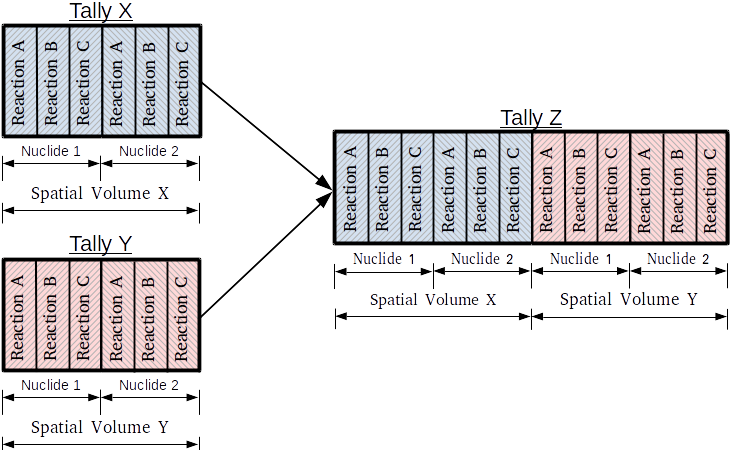
\includegraphics[width=0.6\linewidth]{figures/tally-merge}
  \caption{}
\end{subfigure}
\begin{subfigure}{\textwidth}
  \centering
  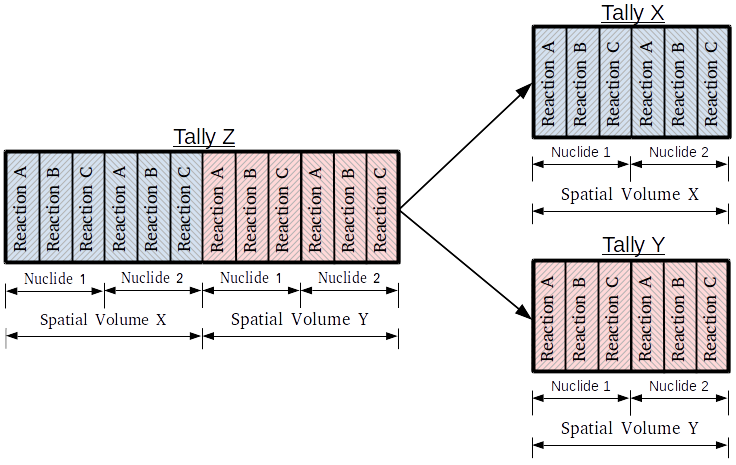
\includegraphics[width=0.6\linewidth]{figures/tally-slice}
  \caption{}
\end{subfigure}
\caption{Two \texttt{Tally} objects for different spatial volumes merged into a single \texttt{Tally} (a). A single \texttt{Tally} is sliced by spatial volume into two distinct \texttt{Tally} objects (b).}
\label{fig:tally-merge-slice}
\end{figure}

%%%%%%%%%%%%%%%%%%%%%%%%%%%%%%%%
\subsubsection{Tally Arithmetic}
\label{subsubsec:tally-arithmetic}

A variety of reaction rate and flux tallies must be arithmetically combined in order to compute MGXS with Monte Carlo. At the most general level, a reaction rate tally must be divided by a flux tally for each energy group, nuclide, and tally volume. The Python API provides a novel feature known as \emph{tally arithmetic} to enable the arithmetic combinations of tallies with efficient vectorized numerical operations across energy groups, nuclides, and spatial tally zones.

Tally arithmetic is an object-oriented data-processing feature that arithmetically combines two or more tallies and/or scalar values into new \emph{derived tallies}. The Python API overloads the \texttt{Tally} class' operators for addition, subtraction, multiplication, and division. Furthermore, the \texttt{Tally} class supports summation and averaging operations across some or all of its filter, nuclide, or score bins.

Multigroup cross sections may be simply and efficiently computed with tally arithmetic. For example, the code snippet in \cref{lst:python-input} illustrates how tally slicing and arithmetic are used to compute a total MGXS. The total MGXS that is returned from the tally division operation is encapsulated within a \texttt{Tally} object. This is the approach used by the MGXS generation module created for OpenMC.

\lstinputlisting[language=Python, basicstyle=\ttfamily\scriptsize, caption={MGXS calculation with tally arithmetic.}, label={lst:python-input}]{listings/tally-arithmetic.py}

Tally arithmetic automatically propagates the uncertainties of the tally operands through the arithmetic operation to estimate the uncertainty of the resulting derived tally. Estimates of the variance for derived tallies are deduced from standard error propagation theory~\cite{bevington2003data}. The division operator is used primarily to compute MGXS from MC tallies. Consider two random variables $X$ and $Y$, generated from distributions with variances $\sigma_{X}^2$ and $\sigma_{Y}^2$, that are divided into a new random variable $Z$ with variance $\sigma_{Z}^2$:

\begin{equation}
\label{eqn:div-prop}
\sigma_{Z}^{2} \approx Z^{2}\left[\left(\frac{\sigma_{X}}{X}\right)^{2} + \left(\frac{\sigma_{Y}}{Y}\right)^{2} - 2\frac{\sigma_{XY}}{Z}\right].
\end{equation}

\noindent The variables $X$ and $Y$ may correspond to reaction rates and the flux tallies, while $Z$ could correspond to the MGXS.

The covariance $\sigma_{XY}$ is not generally computable by using the standard formulation for a tally estimator in a Monte Carlo simulation. Although one could estimate the covariance using ensemble statistics, this approach is typically infeasible. Instead, the covariance term in \cref{eqn:div-prop} is currently neglected by OpenMC's implementation of tally arithmetic. In general, the random variables for reaction rates and fluxes in the same volume of phase space are highly correlated, such that a conservative estimate of the variance for MGXS is obtained by neglecting the covariance.

%%%%%%%%%%%%%%%%%%%%%%%%%%%%%%%%%%%%%
\subsection{Distributed Cell Tallies}
\label{subsec:distribcells}

%Many Monte Carlo codes, including OpenMC, use some variant of combinatorial geometry (CG) because it can represent arbitrary, repeating geometries such as fuel pins and assemblies. However, the CG approach is challenged by applications which require tallies in each instance of a repeated cell throughout a reactor geometry. The ``brute force'' solution is to instantiate a unique cell for each distinct tally zone. However, this defeats the purpose of using CG for its compact representation, and it is not scalable to problems with large tally datasets such as those considered in this thesis.

The \emph{distributed cell tally} algorithm was implemented in OpenMC \cite{lax2014distribcell} to permit simply defined spatial tally zones across repeated cell instances. The distributed cell tally algorithm, abbreviated as the \emph{distribcell} algorithm, may be used to compute spatially varying MGXS across fuel pin cell instances. The distribcell algorithm classifies each unique cell instance using a process that consumes orders of magnitude less memory than would be required by the ``brute force'' approach necessary to accomplish the same objective with other commonly used Monte Carlo codes. Only a single transparent line of XML input is necessary to define a distribcell tally that may span across an arbitrary number of instances for a particular cell. Furthermore, the Python API may be used to perform efficient vectorized transformations of distribcell tally data stored as contiguous NumPy arrays to compute MGXS.

%%%%%%%%%%%%%%%%%%%%%%%%%%%%%%%%%%%%%%%%%%%%%%%%%%%%%%%%%%%%%%%%%%%%%%%%%%%%%%%
\section{MGXS Generation with Monte Carlo}
\label{sec:mgxs-mc}
%%%%%%%%%%%%%%%%%%%%%%%%%%%%%%%%%%%%%%%%%%%%%%%%%%%%%%%%%%%%%%%%%%%%%%%%%%%%%%%


%%%%%%%%%%%%%%%%%%%%%%%%%%%%%%%%%%%%%%%%%%%%%%%%%%%
\subsection{Tally Types Needed for MGXS Generation}
\label{subsec:tally-types}

This section describes how multi-group cross sections may be computed using stochastic integration. In particular, this section outlines the types of OpenMC tallies needed to generate MGXS -- including the scores, filters and estimators for each tally -- and the arithmetic combinations used to combine different tallies.

%%%%%%%%%%%%%%%%%%%%%%%%%%%%%%%%%%%%%%
\subsubsection{Inner Product Notation}
\label{subsubsec:tally-types-notation}

The following sections use angle bracket notation $\langle \cdot , \cdot \rangle$ to represent inner products in phase space. This may correspond to integrals over incoming and/or outgoing energy, space, and angle. Using this notation, a tally estimator for reaction rate $x$ is represented as follows: 

\begin{equation}
\label{eqn:inner-prod}
\langle \Sigma_x, \psi \rangle = \int_{V} \int_{S} \int_{E} \Sigma_{x}(\mathbf{r},E)\psi(\mathbf{r},E,\mathbf{\Omega}) \mathrm{d}E\mathrm{d}\mathbf{\Omega}\mathrm{d}\mathbf{r}
\end{equation}

\noindent This notation is specialized throughout this section with subscripts to indicate the subsets of phase space that are integrated over in the inner product. In particular, subscript $k$ refers to a volume integral over $V_{k}$ for some region of space $k$ for spatial homogenization, while subscript $g$ corresponds to an integral over energies with $E \in [E_{g}, E_{g-1}]$ for energy condensation. For example, the microscopic reaction rate for reaction $x$ by nuclide $i$ is denoted as:

\begin{equation}
\label{eqn:angle-rxn-rate}
\langle \sigma_{x,i}, \psi \rangle_{k,g} = \int_{\mathbf{r} \in V_{k}} \int_{4\pi} \int_{E_{g}}^{E_{g-1}} \sigma_{x,i}(\mathbf{r},E)\psi(\mathbf{r},E,\mathbf{\Omega}) \mathrm{d}E\mathrm{d}\mathbf{\Omega}\mathrm{d}\mathbf{r}
\end{equation}

\noindent The inner product of a function with unity, such as the spatially-homogenized and energy-integrated flux is denoted by:

\begin{equation}
\label{eqn:angle-flux}
\langle \psi \rangle_{k,g} \equiv \langle \psi, \mathbb{1} \rangle_{k,g} = \int_{\mathbf{r} \in V_{k}} \int_{4\pi} \int_{E_{g}}^{E_{g-1}} \psi(\mathbf{r},E,\mathbf{\Omega}) \mathrm{d}E\mathrm{d}\mathbf{\Omega}\mathrm{d}\mathbf{r}
\end{equation}

%Finally, the superscripts $a$ and $t\ell$ are given to those inner products computed with analog and track-length estimators, respectively -- \textit{i.e.}, $\langle \cdot,\cdot \rangle^{a}$ is an analog tally estimator and $\langle \cdot,\cdot \rangle^{t\ell}$ is a track-length tally estimator of the corresponding inner products.

%%%%%%%%%%%%%%%%%%%%%%%%%%%%%%%%%%%%%%%%%%%%%%
\subsubsection{General Reaction Cross Section}
\label{subsubsec:tally-types-gen-xs}

A general spatially-homogenized and energy condensed macroscopic multi-group cross section for reaction $x$, spatial zone $k$ and energy group $g$ is simply the ratio of the group-wise reaction rates $\langle \Sigma_{x}, \psi \rangle_{k,g}$ and fluxes $\langle \psi \rangle_{k,g}$:

\begin{equation}
\label{eqn:general-macro}
\hat{\Sigma}_{x,k,g} = \frac{\langle \Sigma_{x}, \psi \rangle_{k,g}}{\langle \psi \rangle_{k,g}}
\end{equation}

\noindent Likewise, a microscopic MGXS for nuclide $i$ can be computed as follows:

\begin{equation}
\label{eqn:general-micro}
\hat{\sigma}_{x,i,k,g} = \frac{\langle \sigma_{x,i}, \psi \rangle_{k,g}}{\langle \psi \rangle_{k,g}}
\end{equation}

These estimators are used for reaction types which are only dependent on the incoming energy of a neutron, such as total and radiative capture reactions.

%%%%%%%%%%%%%%%%%%%%%%%%%%%%%%%%%%%
\subsubsection{Total Cross Section}
\label{subsubsec:tally-types-tot-xs}

The total macroscopic cross section $\Sigma_{t}$ is a special case of \autoref{eqn:general-micro}, with the total collision rate substituted into the numerator:

\begin{equation}
\label{eqn:total-macro}
\hat{\Sigma}_{t,k,g} = \frac{\langle \Sigma_{t}, \psi \rangle_{k,g}}{\langle \psi \rangle_{k,g}}
\end{equation}

A transport correction is often used to incorporate anisotropic scattering effects into the transport equation with an isotropic scattering kernel. An expression for the in-scatter approximation \cite{yamamoto2008simplified} to the transport correction is computed with an OpenMC tally for the first Legendre scattering moment:

\begin{equation}
\label{eqn:sigs1}
\langle \Sigma_{s1}, \psi \rangle_{k,g'\rightarrow g} = \int_{\mathbf{r} \in V_{k}} \int_{4\pi} \int_{E_{g}}^{E_{g-1}} \int_{E_{g'}}^{E_{g'-1}} \Sigma_{s1}(\mathbf{r},E'\rightarrow E)\psi(\mathbf{r},E',\mathbf{\Omega}) \mathrm{d}E'\mathrm{d}E\mathrm{d}\mathbf{\Omega}\mathrm{d}\mathbf{r}
\end{equation}

\noindent An analog estimator must be used in OpenMC since the tally includes an integral over the outgoing neutron energy. The spatially-homogenized and energy condensed transport-corrected total cross section is computed by summing over all incoming energy groups:

\begin{equation}
\label{eqn:transport-corr-macro}
\hat{\Sigma}_{tr,k,g} = \displaystyle\sum\limits_{g'=1}^{G} \langle{\Sigma_{s1}, \psi \rangle_{k,g'\rightarrow g}}
\end{equation}

\noindent The transport correction is then subtracted from the group-wise total collision rate and normalized by the flux to compute the transport-corrected total cross section:

\begin{equation}
\label{eqn:sigt-transport-macro}
\hat{\tilde{\Sigma}}_{t,k,g} = \frac{\langle \Sigma_{t}, \psi \rangle_{k,g} - \hat{\Sigma}_{tr,k,g}}{\langle \psi \rangle_{k,g}}
\end{equation}

Since the transport correction must be computed using an analog estimator, the total collision and flux in \autoref{eqn:sigt-transport-macro} must also be computed with analog estimators.

%%%%%%%%%%%%%%%%%%%%%%%%%%%%%%%%%%%
\subsubsection{Multiplicity Matrix}
\label{subsubsec:tally-types-mult-mat}

The multiplicity is calculated as

\begin{equation}
\langle \upsilon \sigma_{s,g'\rightarrow g} \phi \rangle = \int_{r \in D} dr \int_{4\pi} d\Omega' \int_{E_{g'}}^{E_{g'-1}} dE' \int_{4\pi} d\Omega \int_{E_g}^{E_{g-1}} dE \; \sum_i \upsilon_i \sigma_i (r, E' \rightarrow E, \Omega' \cdot \Omega) \psi(r, E', \Omega') 
\end{equation}

\begin{equation}
\langle \upsilon \sigma_{s,g'\rightarrow g} \phi \rangle = \int_{r \in D} dr \int_{4\pi} d\Omega' \int_{E_{g'}}^{E_{g'-1}} dE' \int_{4\pi} d\Omega \int_{E_g}^{E_{g-1}} dE \; \sum_i \upsilon_i \sigma_i (r, E' \rightarrow E, \Omega' \cdot \Omega) \psi(r, E', \Omega')
\end{equation}

\begin{equation}
\langle \sigma_{s,g'\rightarrow g} \phi \rangle = \int_{r \in D} dr \int_{4\pi} d\Omega' \int_{E_{g'}}^{E_{g'-1}} dE' \int_{4\pi} d\Omega \int_{E_g}^{E_{g-1}} dE \; \sum_i \upsilon_i \sigma_i (r, E' \rightarrow E, \Omega' \cdot \Omega) \psi(r, E', \Omega') \\
\end{equation}

\begin{equation}
\upsilon_{g'\rightarrow g} = \frac{\langle \upsilon \sigma_{s,g'\rightarrow g} \rangle}{\langle \sigma_{s,g'\rightarrow g} \rangle}
\end{equation}

\noindent where $\upsilon_i$ is the multiplicity for the $i^{th}$ reaction.


%%%%%%%%%%%%%%%%%%%%%%%%%%%%%%%%%%%%%%%%%%%%%
\subsubsection{Scattering Probability Matrix}
\label{subsubsec:tally-types-scatt-prob-mat}


%%%%%%%%%%%%%%%%%%%%%%%%%%%%%%%%%
\subsubsection{Scattering Matrix}
\label{subsubsec:tally-types-scatt-mat}

The isotropic scattering matrix is computed with an inner product of scattering reactions over both incoming and outgoing energies. An analog estimator must be used since the integral is dependent on the neutron's outgoing energy. Similar to the first Legendre moment in \autoref{eqn:sigs1}, the isotropic scattering moment is given by the following expression:

\begin{equation}
\label{eqn:sigs0}
\langle \Sigma_{s0}, \psi \rangle_{k,g'\rightarrow g} = \int_{\mathbf{r} \in V_{k}} \int_{4\pi} \int_{E_{g}}^{E_{g-1}} \int_{E_{g'}}^{E_{g'-1}} \Sigma_{s0}(\mathbf{r},E'\rightarrow E)\psi(\mathbf{r},E,\mathbf{\Omega}) \mathrm{d}E'\mathrm{d}E\mathrm{d}\mathbf{\Omega}\mathrm{d}\mathbf{r}
\end{equation}

\noindent The isotropic scattering matrix is then:

\begin{equation}
\label{eqn:scatt-macro}
\hat{\Sigma}_{s,k,g'\rightarrow g} = \frac{\langle \Sigma_{s0}, \psi \rangle_{k,g'\rightarrow g}}{\langle \psi \rangle_{k,g'}}
\end{equation}

\noindent The transport correction in \autoref{eqn:transport-corr-macro} can be applied by subtracting it from the diagonal elements in the matrix to compute the transport-corrected scattering matrix:

\begin{equation}
\label{eqn:scatt-trans-macro}
\hat{\tilde{\Sigma}}_{s,k,g'\rightarrow g} = \frac{\langle \Sigma_{s0}, \psi \rangle_{k,g'\rightarrow g} - \delta_{g,g'} \hat{\Sigma}_{tr,k,g}}{\langle \psi \rangle_{k,g'}}
\end{equation}

%To incorporate the effect of neutron multiplication from $(n,xn)$ reactions in the above relation, the nu parameter can be set to `True`.

An alternative ``consistent'' form of the scattering matrix can be computed as the product of the scatter cross section and group-to-group scattering probabilities. Unlike the formulation in \autoref{eqn:scatt-macro}, the consistent formulation is computed from the groupwise scattering cross section which uses a track-length estimator. This ensures that reaction rate balance is exactly preserved with a total cross section (\autoref{eqn:total-macro} computed using a tracklength estimator.

For a scattering probability matrix $P_{s,\ell,g'\rightarrow g}$ and scattering cross section $\sigma_s (r, E)$ for incoming energy group $[E_{g'},E_{g'-1}]$ and outgoing energy group $[E_g,E_{g-1}]$, the Legendre scattering moments are calculated as:

\begin{equation}
\label{eqn:scatt-mat-consistent}
\Sigma_{s,\ell,g'\rightarrow g} = \sigma_s (r, E) \times P_{s,\ell,g'\rightarrow g}
\end{equation}

To incorporate the effect of neutron multiplication from $(n,xn)$ reactions ...

\begin{equation}
\label{eqn:nuscatt-mat-consistent}
\sigma_{s,\ell,g'\rightarrow g} = \upsilon_{g'\rightarrow g} \times \sigma_s (r, E) \times P_{s,\ell,g'\rightarrow g}
\end{equation}

Add discussion about consistent scattering formulation ... and about Legendre moments ...

%%%%%%%%%%%%%%%%%%%%%%%%%%%%%%%%%%%%%%%%%%%%%%%%
\subsubsection{Fission Production Cross Section}
\label{subsubsec:tally-types-fiss-prod}

The fission product macroscopic cross section $\nu\Sigma_{f}$ may be treated as a special case of \autoref{eqn:general-micro}, with estimators for the fission production rate and flux:

\begin{equation}
\label{eqn:nu-fiss-macro}
\nu\hat{\Sigma}_{f,k,g} = \frac{\langle \nu\Sigma_{f}, \psi \rangle_{k,g}}{\langle \psi \rangle_{k,g}}
\end{equation}

%%%%%%%%%%%%%%%%%%%%%%%%%%%%%%%%%%%%%%%
\subsubsection{Fission Energy Spectrum}
\label{subsubsec:tally-types-chi}

Unlike the fission production cross section, the fission spectrum is dependent on the outgoing neutron energy and must be computed with analog estimators. The fission production matrix from group $g'$ into group $g$ is given by the following inner product:

\begin{equation}
\label{eqn:nu-fiss-energies}
\langle \nu\Sigma_{f}, \psi \rangle_{k,g'\rightarrow g} = \int_{\mathbf{r} \in V_{k}} \int_{4\pi} \int_{E_{g}}^{E_{g-1}} \int_{E_{g'}}^{E_{g'-1}} \nu\Sigma_{f}(\mathbf{r},E'\rightarrow E)\psi(\mathbf{r},E,\mathbf{\Omega}) \mathrm{d}E'\mathrm{d}E\mathrm{d}\mathbf{\Omega}\mathrm{d}\mathbf{r}
\end{equation}

\noindent The fission spectrum can then be computed from this tally by summing over incoming and outgoing energy groups:

\begin{equation}
\label{eqn:chi}
\hat{\chi}_{k,g} = \frac{\displaystyle\sum\limits_{g'=1}^{G} \langle \nu\Sigma_{f}, \psi \rangle_{k,g'\rightarrow g}}{\displaystyle\sum\limits_{g=1}^{G} \displaystyle\sum\limits_{g'=1}^{G} \langle \nu\Sigma_{f}, \psi \rangle_{k,g'\rightarrow g}}
\end{equation}

\noindent This expression for the fission spectrum will result in a normalized discrete probability distribution for the energy of neutrons emitted from fission.

%%%%%%%%%%%%%%%%%%%%%%%%%%%%%%%%%%%%%%%%
\subsubsection{Delayed Neutron Fraction}
\label{subsubsec:tally-types-beta}

%%%%%%%%%%%%%%%%%%%%%%%%%%%%%%%%%%%%%%%%%%%%%%%%%%%%
\subsubsection{Delayed Neutron Precursor Decay Rate}
\label{subsubsec:tally-types-lambda}

%%%%%%%%%%%%%%%%%%%%%%%%%%%%%%%%%%%%%%%%%%%%%%%%%%%%%%%%
\subsubsection{Delayed Fission Production Cross Section}
\label{subsubsec:tally-types-delay-fiss-prod}

%%%%%%%%%%%%%%%%%%%%%%%%%%%%%%%%
\subsubsection{Inverse Velocity}
\label{subsubsec:tally-types-inv-vel}


%%%%%%%%%%%%%%%%%%%%%%%%%%%%%%%%%%%%%%%%%%%%%%%%%%%
\subsection{Summary}
\label{subsec:tally-types-summary}

The tallies needed to generate MGXS libraries were outlined in detail in the preceding sections, and are summarized in \autoref{tab:tally-types}. The scores and filters correspond to the notation used by the OpenMC code to describe the scoring function and integration bounds. The energy group structure for energy condensation is specified by \texttt{energy} and/or \texttt{energyout} filters in the table. A material, cell, universe or mesh domain is specified by an appropriate filter for spatial homogenization.

\begin{table}[h!]
  \centering
  \caption[Tally types for MGXS generation]{The types of tallies used in MGXS generation with OpenMC.}
  \scriptsize
  \label{tab:tally-types}
  \vspace{6pt}
  \begin{tabular}{ m{2.3cm} m{1.2cm} m{2cm} m{2.5cm} l }
  \toprule
  {\bf Name} &
  {\bf Symbol} &
  {\bf Tally} &
  {\bf Score} &
  {\bf Filters} \\

  \midrule

  \multirow{2}{*}{\bf General} & \multirow{2}{*}{$\Sigma_{x,k,g}$} & $\langle \Sigma_{x}, \psi \rangle_{k,g}$ & reaction $x$ & spatial domain\footnotemark, \texttt{energy} \\
  \cline{3-5}
  & & $\langle \psi \rangle_{k,g}$ & {\texttt{flux}} & spatial domain\ref{foot:domain}, \texttt{energy} \\

  \midrule

  \multirow{2}{*}{\bf Total} & \multirow{2}{*}{$\Sigma_{t,k,g}$} & $\langle \Sigma_{t}, \psi \rangle_{k,g}$ & \texttt{total} & spatial domain, \texttt{energy} \\
  \cline{3-5}
  & & $\langle \psi \rangle_{k,g}$ & \texttt{flux} & spatial domain\ref{domain}, \texttt{energy} \\

  \midrule

  \multirow{3}{*}{\parbox{1.5cm}{\bf Radiative Capture}} & \multirow{3}{*}{$\Sigma_{\gamma,k,g}$} & $\langle \Sigma_{a}, \psi \rangle_{k,g}$ & \texttt{absorption} & spatial domain\ref{foot:domain}, \texttt{energy} \\
  \cline{3-5}
  & & $\langle \Sigma_{f}, \psi \rangle_{k,g}$ & \texttt{fission} & spatial domain\ref{foot:domain}, \texttt{energy} \\
  \cline{3-5}
  & & $\langle \psi \rangle_{k,g}$ & \texttt{flux} & spatial domain\ref{foot:domain}, \texttt{energy} \\

  \midrule

  \textbf{\parbox{1.5cm}{\bf Transport Correction}} & $\Sigma_{tr,k,g}$ & $\langle \Sigma_{s1}, \psi \rangle_{k,g'\rightarrow g}$ & \texttt{(nu-)scatter-0} & spatial domain\ref{foot:domain}, \texttt{energyout} \\

  \midrule

  \multirow{2}{*}{\parbox{1.5cm}{\bf Scattering Matrix}} & \multirow{2}{*}{$\Sigma_{s,k,g'\rightarrow g}$} & $\langle \Sigma_{s0}, \psi \rangle_{k,g'\rightarrow g}$ & \texttt{(nu-)scatter-0} & spatial domain\ref{foot:domain}, \texttt{energy}, \texttt{energyout} \\
  \cline{3-5}
  & & $\langle \psi \rangle_{k,g}$ & \texttt{flux} & spatial domain\ref{foot:domain}, \texttt{energy} \\

  \midrule

  \multirow{2}{*}{\parbox{1.5cm}{\bf Fission \hspace{1cm} Production}} & \multirow{2}{*}{$\nu\Sigma_{f,k,g}$} & $\langle \nu\Sigma_{f}, \psi \rangle_{k,g}$ & \texttt{nu-fission} & spatial domain\ref{foot:domain}, \texttt{energy} \\
  \cline{3-5}
  & & $\langle \psi \rangle_{k,g}$ & \texttt{flux} & spatial domain\ref{foot:domain}, \texttt{energy} \\

  \midrule
  
  \parbox{1.5cm}{\parbox{1.2cm}{\bf Fission Spectrum}} & $\chi_{k,g}$ & $\langle \nu\Sigma_{f}, \psi \rangle_{k,g'\rightarrow g}$ & \texttt{nu-fission} & spatial domain\ref{foot:domain}, \texttt{energy}, \texttt{energyout} \\

  \midrule

  \parbox{1.5cm}{\parbox{1.9cm}{\bf Delayed Fission Spectrum}} & & & \\

  \midrule

  \parbox{1.5cm}{\parbox{2.3cm}{\bf Delayed Prescursor Decay Rate}} & & & \\

  \midrule

  \parbox{1.5cm}{\parbox{2cm}{\bf Delayed Neutron Fraction}} & & & \\

  \midrule

  \parbox{1.5cm}{\parbox{1.2cm}{\bf Inverse Velocity}} & & & \\

  \midrule

\end{tabular}
\end{table}

\footnotetext{\label{foot:domain} A \texttt{material}, \texttt{cell}, \texttt{distribcell}, \texttt{universe} or \texttt{mesh} filter.}


%%%%%%%%%%%%%%%%%%%%%%%%%%%%%
\subsection{Tally Estimators}
\label{subsec:tally-est}

\begin{itemize}[noitemsep]
\item Table of the tally estimators acceptable for each MGXS type
\item Mention tally estimators can be toggled? Or discuss in software design?
\item Add footnote mentioning consistent scattering formulation
\end{itemize}

\begin{table}[h!]
  \centering
  \caption{The tally estimators supported by each MGXS type.}
  \small
  \label{tab:mgxs-tally-estimators} 
  \vspace{6pt}
  \begin{tabular}{l c c}
  \toprule
  \textbf{Class} &
  \textbf{Analog} &
  \textbf{Track-length} \\
  \midrule
  \multicolumn{3}{c}{\bf Prompt Neutron Constants} \\
  \midrule
  \texttt{AbsorptionXS} & \cmark & \cmark \\
  \texttt{CaptureXS} & \cmark & \cmark \\
  \texttt{Chi} & \cmark & \xmark \\
  \texttt{FissionXS} & \cmark & \cmark \\
  \texttt{InverseVelocity} & \cmark & \xmark \\
  \texttt{KappaFissionXS} & \cmark & \cmark \\
  \texttt{MultiplicityMatrixXS} & \cmark & \xmark \\
  \texttt{NuFissionMatrixXS} & \cmark & \xmark \\
  \texttt{ScatterXS} & \cmark & \cmark \\
  \texttt{ScatterMatrixXS} & \cmark & \xmark \\
  \texttt{ScatterProbabilityMatrixXS} & \cmark & \xmark \\
  \texttt{TotalXS} & \cmark & \xmark \\
  \texttt{TransportXS} & \cmark & \xmark \\
  \midrule
  \multicolumn{3}{c}{\bf Delayed Neutron Constants} \\
  \midrule
  \texttt{Beta} & \cmark & \xmark \\
  \texttt{ChiDelayed} & \cmark & \xmark \\
  \texttt{DelayedNuFissionXS} & \cmark & \xmark \\
  \texttt{DecayRate} & \cmark & \xmark \\
  \bottomrule
\end{tabular}
\end{table}

%%%%%%%%%%%%%%%%%%%%%%%%%%%%%%%%%%%%%%%%%%%%%%%%%%%%%%%%%%%%%%%%%%%%%%%%%%%%%%%
\section{Software Design}
\label{sec:software}
%%%%%%%%%%%%%%%%%%%%%%%%%%%%%%%%%%%%%%%%%%%%%%%%%%%%%%%%%%%%%%%%%%%%%%%%%%%%%%%

The OpenMC Python API's \texttt{openmc.mgxs} module was designed to generate multi-group cross sections. The \texttt{openmc.mgxs} module is built atop the underlying core features in the rest of the API to support a seamless interface for both input generation and downstream data processing of MGXS from Python. In particular, one may specify the MGXS to compute and the \texttt{openmc.mgxs} module will construct the necessary \texttt{Tally} objects. The \texttt{Tally} objects may be easily exported to XML input files for OpenMC, and used to containerize and process the tally data produced by an OpenMC simulation. The \texttt{openmc.mgxs} module thereby leverages the software stack (\textit{e.g.}, tally arithmetic, Pandas DataFrames) provided by the Python API.

The \texttt{openmc.mgxs} module uses an object-oriented design based on an abstract \texttt{MGXS} class with subclasses for different reaction types. The \texttt{MGXS} subclasses are itemized in \autoref{tab:mgxs-types} and compute macroscopic or microscopic multi-group constants in one or more arbitrary energy group structures from MC tallies. The \texttt{openmc.mgxs} module also includes a \texttt{Library} class which automates the construction of \texttt{MGXS} objects for different group structures, spatial domains, and reaction types.

\begin{table}[h!]
  \centering
  \caption{The multi-group cross section types implemented by the \texttt{openmc.mgxs} module.}
  \small
  \label{tab:mgxs-types} 
  \vspace{6pt}
  \begin{tabular}{l l}
  \toprule
  \textbf{Class} &
  \textbf{Description} \\
  \midrule
  \texttt{AbsorptionXS} & Absorption \\
  \texttt{CaptureXS} & Radiative capture \\
  \texttt{Chi} & Fission emission spectrum \\
  \texttt{FissionXS} & Fission \\
  \texttt{InverseVelocity} & Inverse neutron velocity \\
  \texttt{KappaFissionXS} & Fission energy release \\
  \texttt{MultiplicityMatrixXS} & Scattering multiplicity matrix \\
  \texttt{NuFissionMatrixXS} & Fission production matrix \\
  \texttt{ScatterXS} & Scattering \\
  \texttt{ScatterMatrixXS} & Scattering matrix \\
  \texttt{ScatterProbabilityMatrixXS} & Scattering probability matrix \\
  \texttt{TotalXS} & Total collision \\
  \texttt{TransportXS} & Transport-corrected total collision \\
  \bottomrule
\end{tabular}
\end{table}


%%%%%%%%%%%%%%%%%%%%%%%%%%%%%
\subsection{XML Input Generation}
\label{subsec:xml-inputs}

%\begin{itemize}[noitemsep]
%\item workflow: create Python model, create \texttt{Library}, export to XML
%\item code snippet?
%\end{itemize}

%%%%%%%%%%%%%%%%%%%%%%%%%%%%%
\subsection{Data Processing}
\label{subsec:xml-inputs}

\begin{itemize}[noitemsep]
\item refer to PyAPI features that are ``inherited'' by \texttt{openmc.mgxs}:
  \begin{itemize}[noitemsep]
  \item Pandas DataFrames, tally arithmetic/slicing/merging, ...
  \end{itemize}
\end{itemize}

%%%%%%%%%%%%%%%%%%%%%%%%%
\subsection{Data Storage}
\label{subsec:xml-inputs}

The \texttt{openmc.mgxs} module was developed with general design principles to generate MGXS for any multi-group neutron transport code. Although the module does not explicitly support any multi-group codes, it can export MGXS data to a variety of data storage formats, including Comma-Separated Values (CSV) and HDF5. The exported MGXS files may be easily transformed into the database or input files required by a particular multi-group code.
%%%%%%%%%%%%%%%%%%%%%%%%%%%%%%%%%%%%%%%%%%%%%%%%%%%%%%%%%%%%%%%%%%%%%%%%%%%%%%%
\section{Features}
\label{sec:features}
%%%%%%%%%%%%%%%%%%%%%%%%%%%%%%%%%%%%%%%%%%%%%%%%%%%%%%%%%%%%%%%%%%%%%%%%%%%%%%%


%%%%%%%%%%%%%%%%%%%%%%%%%%%%%%%%%%%%%%%%%%%%
\subsection{Energy Condensation}
\label{subsec:energy-condense}

The \texttt{MGXS.get_condensed_xs(...)} method


%%%%%%%%%%%%%%%%%%%%%%%%%%%%%%%%%%%%%%%%%%%%
\subsection{Pin-Wise Spatial Homogenization}
\label{subsec:pinwise-homogenize}

The \texttt{MGXS.get_subdomain_avg_xs(...)} method


%%%%%%%%%%%%%%%%%%%%%%%%%%%%%%%%%%%%%%%%%%%%
\subsection{Microscopic MGXS}
\label{subsec:micro-macro}

Ummm, I hear it is unique that we can calculate micros?


%%%%%%%%%%%%%%%%%%%%%%%%%%%%%%%
\subsection{Scattering Moments}
\label{subsec:scatt-moments}

Up to tenth order scattering moment matrices.


%%%%%%%%%%%%%%%%%%%%%%%%%%%%%%%%%%%%%%%%
\subsection{Isotropic in Lab Scattering}
\label{subsec:iso-in-lab}

For benchmarking with isotropic multi-group codes. Also useful more generally to quantify the impact of anisotropic scattering sources.

%%%%%%%%%%%%%%%%%%%%%%%%%%%%%%%%%%%%%%%%%%%%%%%%%%%%%%%%%%%%%%%%%%%%%%%%%%%%%%%
\section{Conclusions}
\label{sec:conclusions}
%%%%%%%%%%%%%%%%%%%%%%%%%%%%%%%%%%%%%%%%%%%%%%%%%%%%%%%%%%%%%%%%%%%%%%%%%%%%%%%

Monte Carlo methods are increasingly used to generate multigroup cross sections for coarse mesh neutron diffusion codes. This paper introduced the \texttt{openmc.mgxs} Python module to generate MGXS with the OpenMC Monte Carlo code for neutron transport applications. This new module utilizes OpenMC's tally system to perform stochastic integration of reaction rates and fluxes for a user-specified energy group discretization and spatial mesh. The different types of MGXS computable to date---including standard group-wise constants, as well as prompt and delayed constants---were tabulated here. The \texttt{openmc.mgxs} module leverages OpenMC's Python API, along with its support for tally slicing, merging, and arithmetic, to provide a scalable data-processing framework complementary to but separate from the transport kernel implemented in the OpenMC executable.

A case study used the multigroup OpenMOC transport code with 70-group MGXS generated by OpenMC to model two heterogeneous PWR benchmarks. The study showed that OpenMOC predicted eigenvalues to within 50 pcm and fission rates to within 1\% of reference solutions computed by OpenMC, demonstrating the efficacy of the \texttt{openmc.mgxs} module to enable highly accurate multigroup transport calculations. \textcolor{red}{The multi-group constants generated by OpenMC are intended for use by fine-mesh transport rather than coarse-mesh diffusion codes, which brings its own set of unique -- though not mutually exclusive -- challenges with respect to few-group diffusion.} We expect that \texttt{openmc.mgxs} may prove to be a useful platform for research to address these challenges for MC-based MGXS generation in the future.

%A fine spatial and/or energy discretization may be used by OpenMC to tabulate MGXS, and subsequently condensed in energy and/or homogenized in space with data processing features in Python.

%%%%%%%%%%%%%%%%%%%%%%%%%%%%%%%%%%%%%%%%%%%%%%%%%%%%%%%%%%%%%%%%%%%%%%%%%%%%%%%
\section*{Acknowledgments}
%%%%%%%%%%%%%%%%%%%%%%%%%%%%%%%%%%%%%%%%%%%%%%%%%%%%%%%%%%%%%%%%%%%%%%%%%%%%%%%


%\section*{References}
\setlength{\baselineskip}{12pt}
\bibliography{references}
\bibliographystyle{ans}

\end{document}
